\section{Spatial augmented reality}\label{sec:sar}

Projection mapping is a \gls{sar} \cite{Bimber2005} approach in which video projectors are used to overlay virtual geometry on top of real objects or surfaces. This allows to create an immersive environment that together with 3D perception systems can be used to develop interactive interfaces that show contextual information for helping or teaching human operators performing complex tasks faster. The next sections describe the mathematical modeling of video projectors within \gls{opengl} and the associated calibration that is necessary for performing proper 3D rendering of the virtual world in order to achieve high accuracy projection.


\subsection{Projector modeling}

Over the years, several projection technologies were developed according to the requirements of color fidelity / saturation, image sharpness, brightness, contrast, refresh rate and price. Currently, the video projection market is split between reflective \gls{dlp} and transmissive \gls{lcd} projection technology, with a small percentage of projectors consisting of a hybrid between the two technologies (\gls{lcos}).

For video projection mapping purposes, reflective projectors are better suited than the remaining technologies given their ability to create images with smaller gaps between the projected pixels (smoother images) and they also have higher contrast, better color accuracy / uniformity, much fewer dead pixels and the image quality does not degrade over time. The main stages of the image creation in a \gls{dlp} projector are show in \cref{fig:dlp-projector-diagram-dmd}. The first phase is the generation of light from either a lamp or a \gls{led} / laser array, which is later on condensed on a lens in order to pass through a moving color wheel to become one of the 3 primary additive colors (red, green, blue). The colored light then passes through a shaping lens and hits a \gls{dmd} which has an electronic controllable mirror for each projection pixel that either reflects the light into the projection lens or into a heat sink. Color shading is achieved by controlling how long and how often the micro mirrors in the \gls{dmd} are reflecting each light color into the lens or into the heat sink.

The mathematical modeling of a \gls{dlp} projector can be seen as an inverse pinhole camera (diagram shown in \cref{fig:camera-intrinsics-2}) due to the grid disposition of the mirrors in the \gls{dmd} and the very low distortion that modern \gls{dlp} projectors have. As such, rendering of 3D virtual environments can be performed efficiently using an extended version of the \gls{opengl} projection matrix\footnote{\url{http://ksimek.github.io/2013/06/03/calibrated\_cameras\_in\_opengl}} (presented in \cref{eq:projection-matrix}).

The perspective projection of vertex data is one of the pivotal stages in any rendering engine and is responsible from converting 3D geometry from the camera space into the clipping space (as depicted in \cref{fig:opengl-mvp,fig:gl-projection-matrix}). This matrix is usually created using the $glOrtho$ function (matrix shown in \cref{eq:glOrtho}) for orthographic projection or the $glFrustum$ (matrix presented in \cref{eq:glFrustum}) for perspective projection. Looking at both matrices, we can see that the $glFrustum$ can be decomposed to include the $glFrustum$ matrix and a $Q$ matrix (shown in \cref{eq:Q}) that corresponds to the intrinsic parameters of a pinhole camera with the same focal length for the X and Y axis, the principal point at the center of the image and no axis skew. The main difference between the $Q$ matrix and the traditional $K$ matrix \cite{Hartley2003} (shown in \cref{eq:k}) is the bottom row of $Q$, in which the $w$ component of the homogeneous matrix was set to the -Z coordinate. This is a matrix optimization associated with the perspective z-divide that is required to convert 4D homogeneous coordinates to 3D Cartesian coordinates. It has a negative sign because by default the \gls{opengl} camera is setup to look along the -Z axis (as can be seen in \cref{fig:gl-projection-matrix}), and to simplify and optimize the calculations using the similar triangles properties (displayed in \cref{fig:similar-triangles}), the Z coordinate needs to be negated for having a positive value. Looking at \cref{eq:k2}, it can be seen that $K$ can be easily adapted to take this implementation detail into consideration, which allows to extend the $Q$ matrix with the intrinsics parameters estimated by the OpenCV $calib3d$ module. Namely, $Q$ can be extended (as shown in \cref{eq:q2}) to support pinhole cameras with different focal lengths for the X and Y axis ($Fx$ and $Fy$), have an arbitrary axis skew ($S$) and non-centered principal point ($Cx$ and $Cy$). Moreover, the $glOrtho$ matrix can be simplified for this particular use case (as seen in \cref{eq:glOrtho2}), in order to optimize the creation of the extended \gls{opengl} perspective projection matrix that takes into consideration the full camera intrinsics shown in \cref{eq:k}. This extension to the default \gls{opengl} projection matrix is of critical importance for being able to model video projectors as \gls{opengl} cameras, because unlike normal cameras that have the principal point close the image center, video projectors have the principal point at the bottom of the image. As such, \gls{sar} systems must take great care when generating the image that will be projected, otherwise the overlap error between the physical and virtual objects will be too much for making the system usable. The correction of lens distortion typically uses 3 coefficients for removing radial distortions and 2 coefficients for accounting for the tangential distortions. Even thought being relatively small in \gls{dlp} projectors, they can be removed in a post-processing stage after 3D rendering or using a shader in the new \gls{opengl} \gls{api}.

\begin{figure}[!ht]
	\centering
	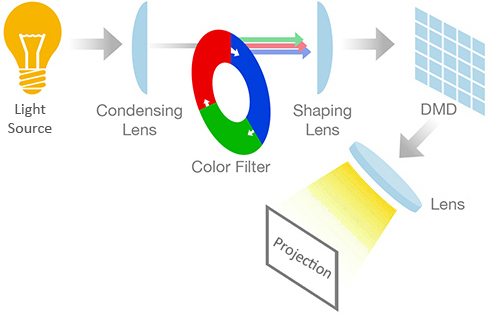
\includegraphics[height=.13\textheight]{dlp-projector-diagram-dmd}
	\caption[Single chip \glsentrytext{dlp} diagram]{Single chip \glsentrytext{dlp} diagram\protect\footnotemark}
	\label{fig:dlp-projector-diagram-dmd}
\end{figure}

\begin{figure}[!ht]
	\centering
	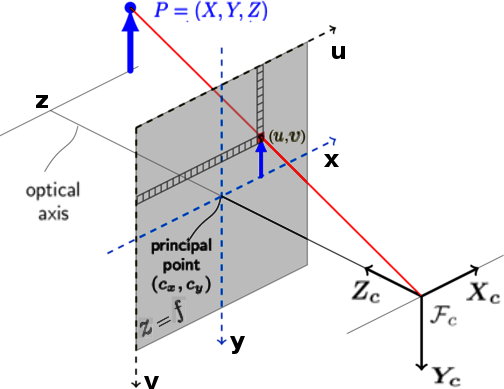
\includegraphics[height=.185\textheight]{camera-intrinsics-2}
	\caption[Pinhole camera model used in OpenCV calib3d module]{Pinhole camera model used in OpenCV calib3d module\protect\footnotemark}
	\label{fig:camera-intrinsics-2}
\end{figure}

\begin{figure}[!ht]
	\centering
	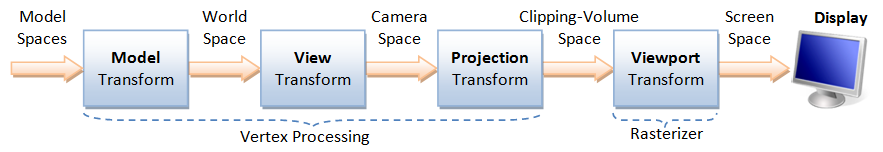
\includegraphics[width=.98\textwidth]{opengl-mvp}
	\caption[OpenGL rendering pipeline]{OpenGL rendering pipeline\protect\footnotemark}
	\label{fig:opengl-mvp}
\end{figure}

\begin{figure}[!ht]
	\centering
	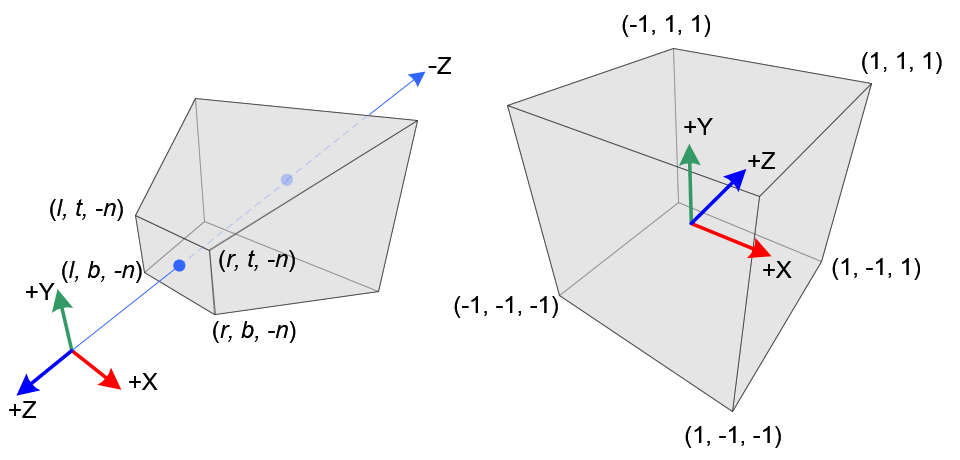
\includegraphics[height=.12\textheight]{gl-projection-matrix}
	\caption[{\glsentrytext{opengl} perspective frustum (left) with the associated \glsentrytext{ndc} cube}]{{\glsentrytext{opengl} perspective frustum (left) with the associated \glsentrytext{ndc} cube}\protect\footnotemark}
	\label{fig:gl-projection-matrix}
\end{figure}

\begin{figure}[!ht]
	\centering
	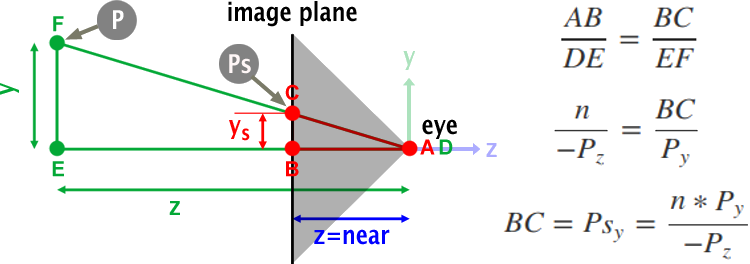
\includegraphics[width=.7\textwidth]{similar-triangles}
	\caption[Similar triangles properties diagram]{Similar triangles properties diagram\protect\footnotemark}
	\label{fig:similar-triangles}
\end{figure}

\footnotetext[\numexpr\value{footnote}-4]{\url{https://vimeo.com/blog/post/display-tech-home-projectors}}
\footnotetext[\numexpr\value{footnote}-3]{\url{https://docs.opencv.org/master/d9/d0c/group__calib3d.html}}
\footnotetext[\numexpr\value{footnote}-2]{\url{https://www.ntu.edu.sg/home/ehchua/programming/opengl/CG_BasicsTheory.html}}
\footnotetext[\numexpr\value{footnote}-1]{\url{http://www.songho.ca/opengl/gl_projectionmatrix.html}}
\footnotetext[\value{footnote}]{\url{http://www.scratchapixel.com/lessons/3d-basic-rendering/perspective-and-orthographic-projection-matrix/opengl-perspective-projection-matrix}}


{
	\setlength\arraycolsep{.15em}
	\scriptsize

	\begin{equation}\label{eq:glOrtho}
		glOrtho{=}
		\begin{bmatrix}
			\vfrac{2}{Right - Left} & 0 & 0 & -\vfrac{Right + Left}{Right - Left} \\[\smallskipamount]
			0 & \vfrac{2}{Top - Bottom} & 0 & -\vfrac{Top + Bottom}{Top - Bottom} \\[\smallskipamount]
			0 & 0 & -\vfrac{2}{Far - Near} & -\vfrac{Far + Near}{Far - Near} \\[\smallskipamount]
			0 & 0 & 0 & 1
		\end{bmatrix}
	\end{equation}

	\begin{equation}\label{eq:Q}
		Q{=}
		\begin{bmatrix}
			Near & 0 & 0 & 0 \\[\smallskipamount]
			0 & Near & 0 & 0 \\[\smallskipamount]
			0 & 0 & Near + Far & Near \times Far \\[\smallskipamount]
			0 & 0 & -1 & 0
		\end{bmatrix}
	\end{equation}

	\begin{equation}\label{eq:glFrustum}
		\begin{split}
			glFrustum = PerspectiveProjectionMatrix = glOrtho \times Q
			\\=
			\begin{bmatrix}
				\vfrac{2 \times Near}{Right - Left} & 0 & \vfrac{Right + Left}{Right - Left} & 0 \\[\smallskipamount]
				0 & \vfrac{2 \times Near}{Top - Bottom} & \vfrac{Top + Bottom}{Top - Bottom} & 0 \\[\smallskipamount]
				0 & 0 & -\vfrac{Far + Near}{Far - Near} & -\vfrac{2 \times Far \times Near}{Far - Near} \\[\smallskipamount]
				0 & 0 & -1 & 0
			\end{bmatrix}
		\end{split}
	\end{equation}

	\begin{equation}\label{eq:k}
		K{=}
		\begin{bmatrix}
			Fx & S & Cx & 0 \\[\smallskipamount]
			0 & Fy & Cy & 0 \\[\smallskipamount]
			0 & 0 & 1 & 0
		\end{bmatrix}
	\end{equation}
	
	\begin{equation}\label{eq:k2}
		K'{=}
		K
		\times
		\begin{bmatrix}
		1 & 0 & 0 & 0 \\[\smallskipamount]
		0 & 1 & 0 & 0 \\[\smallskipamount]
		0 & 0 & -1 & 0 \\[\smallskipamount]
		0 & 0 & 0 & 1
		\end{bmatrix}
		=
		\begin{bmatrix}
		Fx & S & -Cx & 0 \\[\smallskipamount]
		0 & Fy & -Cy & 0 \\[\smallskipamount]
		0 & 0 & -1 & 0
		\end{bmatrix}
	\end{equation}

	\begin{equation}\label{eq:q2}
		Q'{=}
		\begin{bmatrix}
			Fx & S & -Cx & 0 \\[\smallskipamount]
			0 & Fy & -Cy & 0 \\[\smallskipamount]
			0 & 0 & Near + Far & Near \times Far \\[\smallskipamount]
			0 & 0 & -1 & 0
		\end{bmatrix}
	\end{equation}

	\begin{equation}\label{eq:glOrtho2}
		glOrtho'{=}
		\begin{bmatrix}
			\vfrac{2}{IWidth} & 0 & 0 & -1 \\[\smallskipamount]
			0 & \vfrac{2}{IHeight} & 0 & -1 \\[\smallskipamount]
			0 & 0 & -\vfrac{2}{Far - Near} & -\vfrac{Far + Near}{Far - Near} \\[\smallskipamount]
			0 & 0 & 0 & 1
		\end{bmatrix}
	\end{equation}

	\begin{equation}\label{eq:projection-matrix}
		ExtendedOpenGLPerspectiveProjectionMatrix = glOrtho' \times Q'
	\end{equation}
}


\subsection{Projector calibration}

High accuracy projection mapping requires proper hardware / software calibration of the camera / projector and also appropriate positioning within the intended workspace in order to avoid occlusions caused by the objects 3D shape or the human operators. This calibration estimates the intrinsic parameters of the projector (that do not change when the projector is moved within the workspace) along with the extrinsic parameters that are needed to know where is the projector in the global reference frame in order to be able to do proper 3D rendering of the scene that will be projected.

The intrinsic parameters of a \gls{dlp} projector can be computed using image analysis of complementary gray code patterns (example in \cref{fig:dlp-calibration-pattern-wall}) projected into a chessboard. The calibration system proposed in \cite{Moreno2012} was used to retrieve the 5 intrinsic parameters (Fx, Fy, Cx, Cy, S) of the projector along with the 3D position and rotation of the projector in relation to the camera (that remains firmly attached to the projector support for fast recalibration of the extrinsic parameters, as seen in \cref{fig:hardware}). It was used 5 sets of 42 gray code image patterns captured with the chessboard in different positions and orientations in relation to the projector, that was pointing to the table workspace at a distance of 0.81 meters. After calibration, it was projected a validation pattern to evaluate the accuracy of the projection, and as can be seen in \cref{fig:dlp-projected-chessboard}, the white squares were projected into the chessboard with sub-millimeter accuracy.

\begin{figure}[H]
	\begin{floatrow}[2]
		\ffigbox[\FBwidth]
		{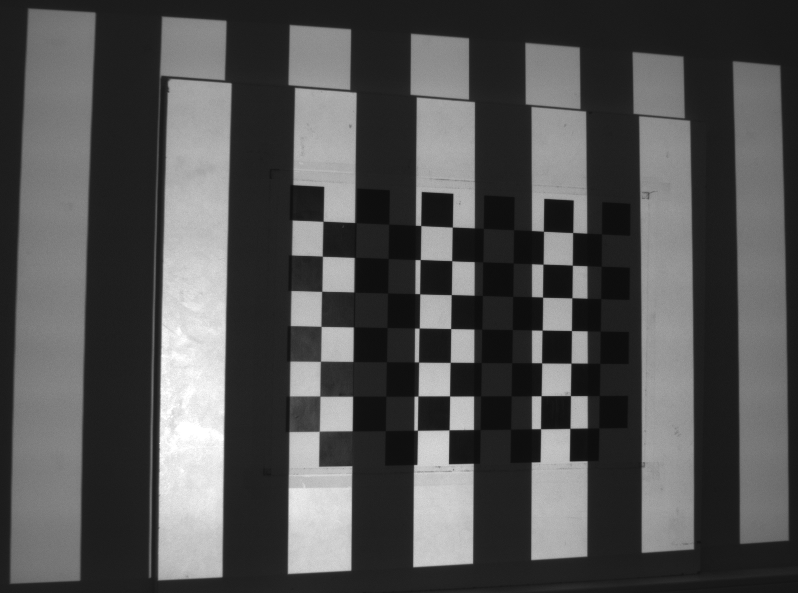
\includegraphics[height=.124\textheight]{dlp-calibration-pattern-wall}}
		{\caption{One of the \glsentrytext{dlp} projector calibration patterns}\label{fig:dlp-calibration-pattern-wall}}
		\ffigbox[\FBwidth]
		{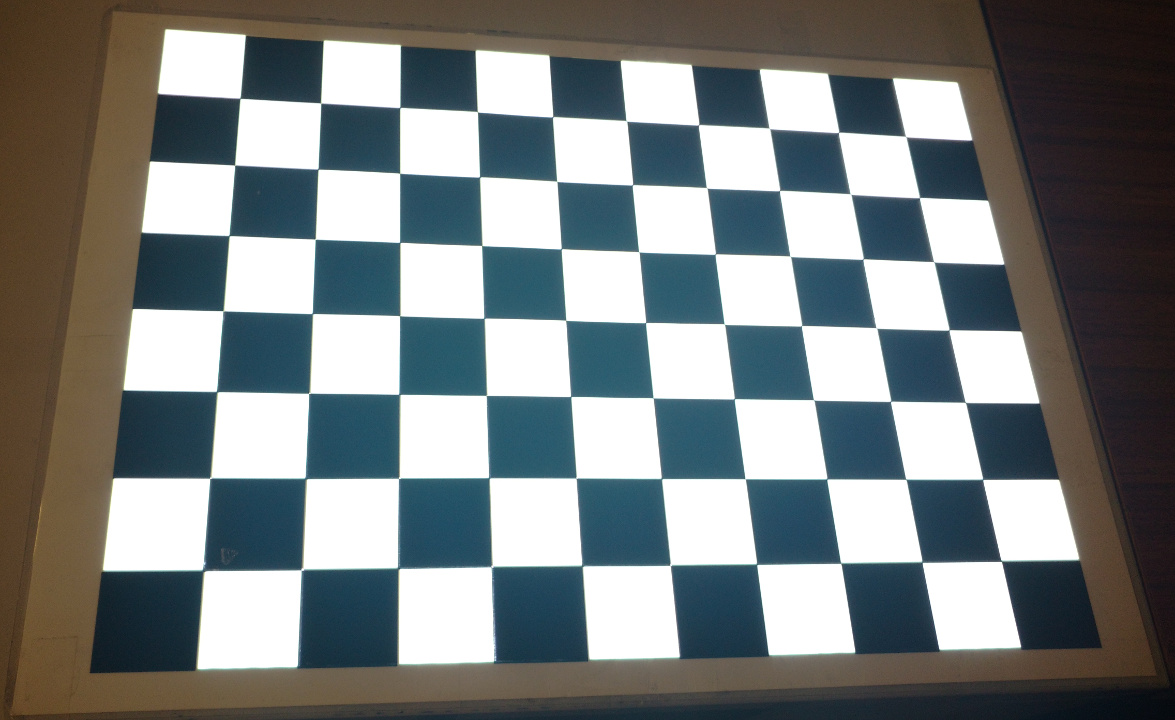
\includegraphics[height=.124\textheight]{chessboard}}
		{\caption{\glsentrytext{dlp} projector validation pattern}\label{fig:dlp-projected-chessboard}}
	\end{floatrow}
\end{figure}

After having the intrinsic parameters of the camera and projector along with the relative position of the projector in relation to the camera, computing the global position of the projector in relation to the chessboard reference frame can be done by multiplying the $4 \times 4$ homogeneous matrix that gives the transformation from the chessboard origin to the camera frame, with the $4 \times 4$ homogeneous matrix that gives the transformation from the camera frame to the projector frame.

%\begin{figure}[H]
%	\centering
%	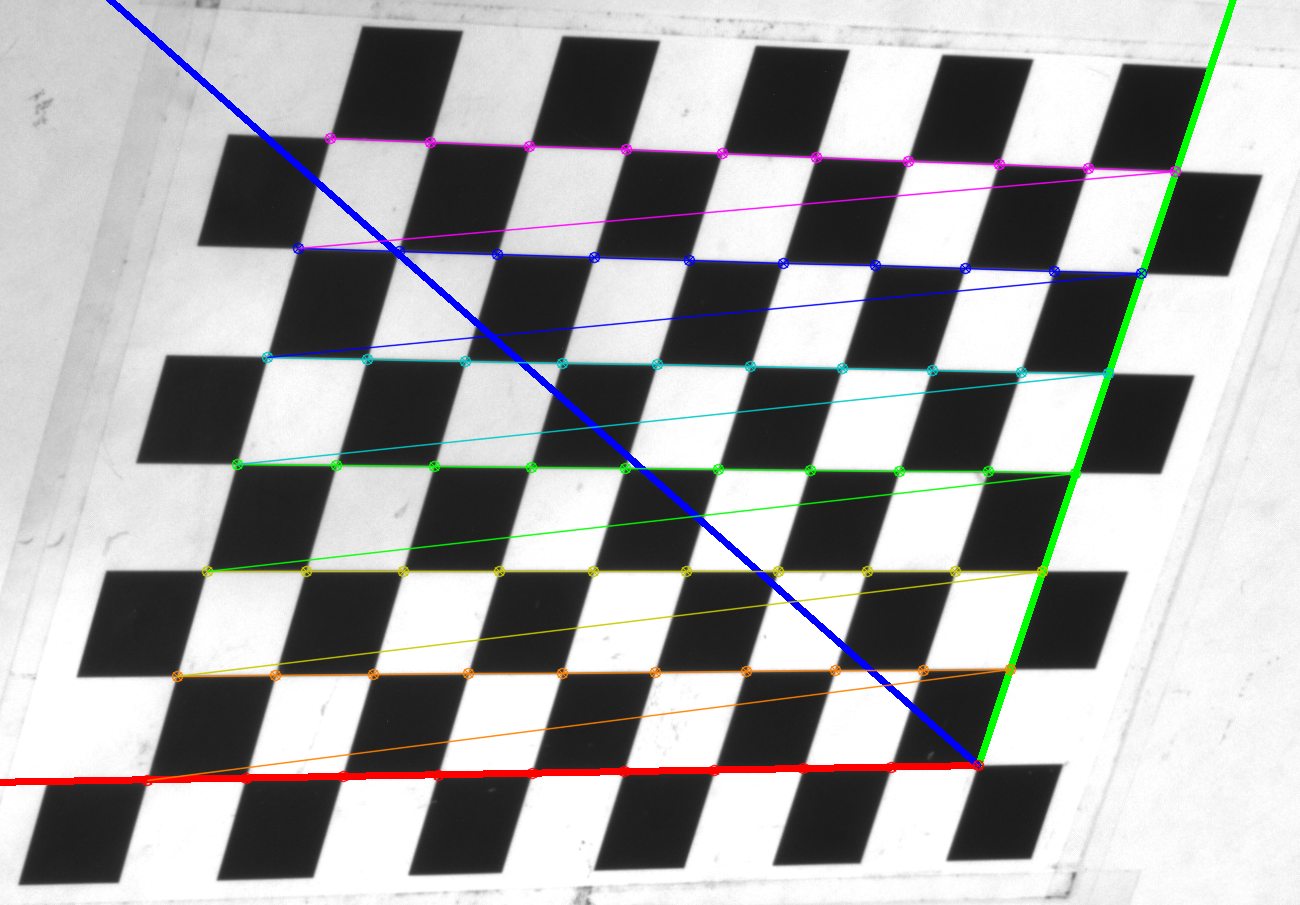
\includegraphics[width=0.47\linewidth]{chess-board-detection}
%	\caption{Camera pose estimation in relation to the chessboard origin (using the Kinect 2 RGB camera)}
%	\label{fig:chess-board-detection}
%\end{figure}


\subsection{Scene rendering}

For achieving accurate projection mapping, the Gazebo simulator\footnote{\url{http://gazebosim.org}} camera implementation was improved to allow the setting of a custom projection matrix in order to perform 3D rendering with a camera model that takes into account the projector intrinsic parameters. Moreover, it was added the possibility to dynamically change image, video and text during runtime for allowing the display of the relevant information for each assembly step.
For efficient 3D scene rendering, the Gazebo simulator relies on the cross platform open source Ogre3D graphics engine\footnote{\url{http://www.ogre3d.org}}, that in turn uses the \gls{opengl} \gls{gpu} \gls{api} to take advantage of the massively parallel graphics cards currently available to generate raster images for the \gls{dlp} projector (example of a rendered scene for the last assembly step in \cref{fig:scene-rendering}).

For user interface, the Gazebo simulator has a Qt\footnote{\url{https://www.qt.io}} \gls{gui} that allows visual inspection of the scene while also giving the option to add new objects or move and rotate existing models. Moreover, for lightweight rendering, it can also start in server mode without a \gls{gui}.

\begin{figure}[ht]
	\centering
	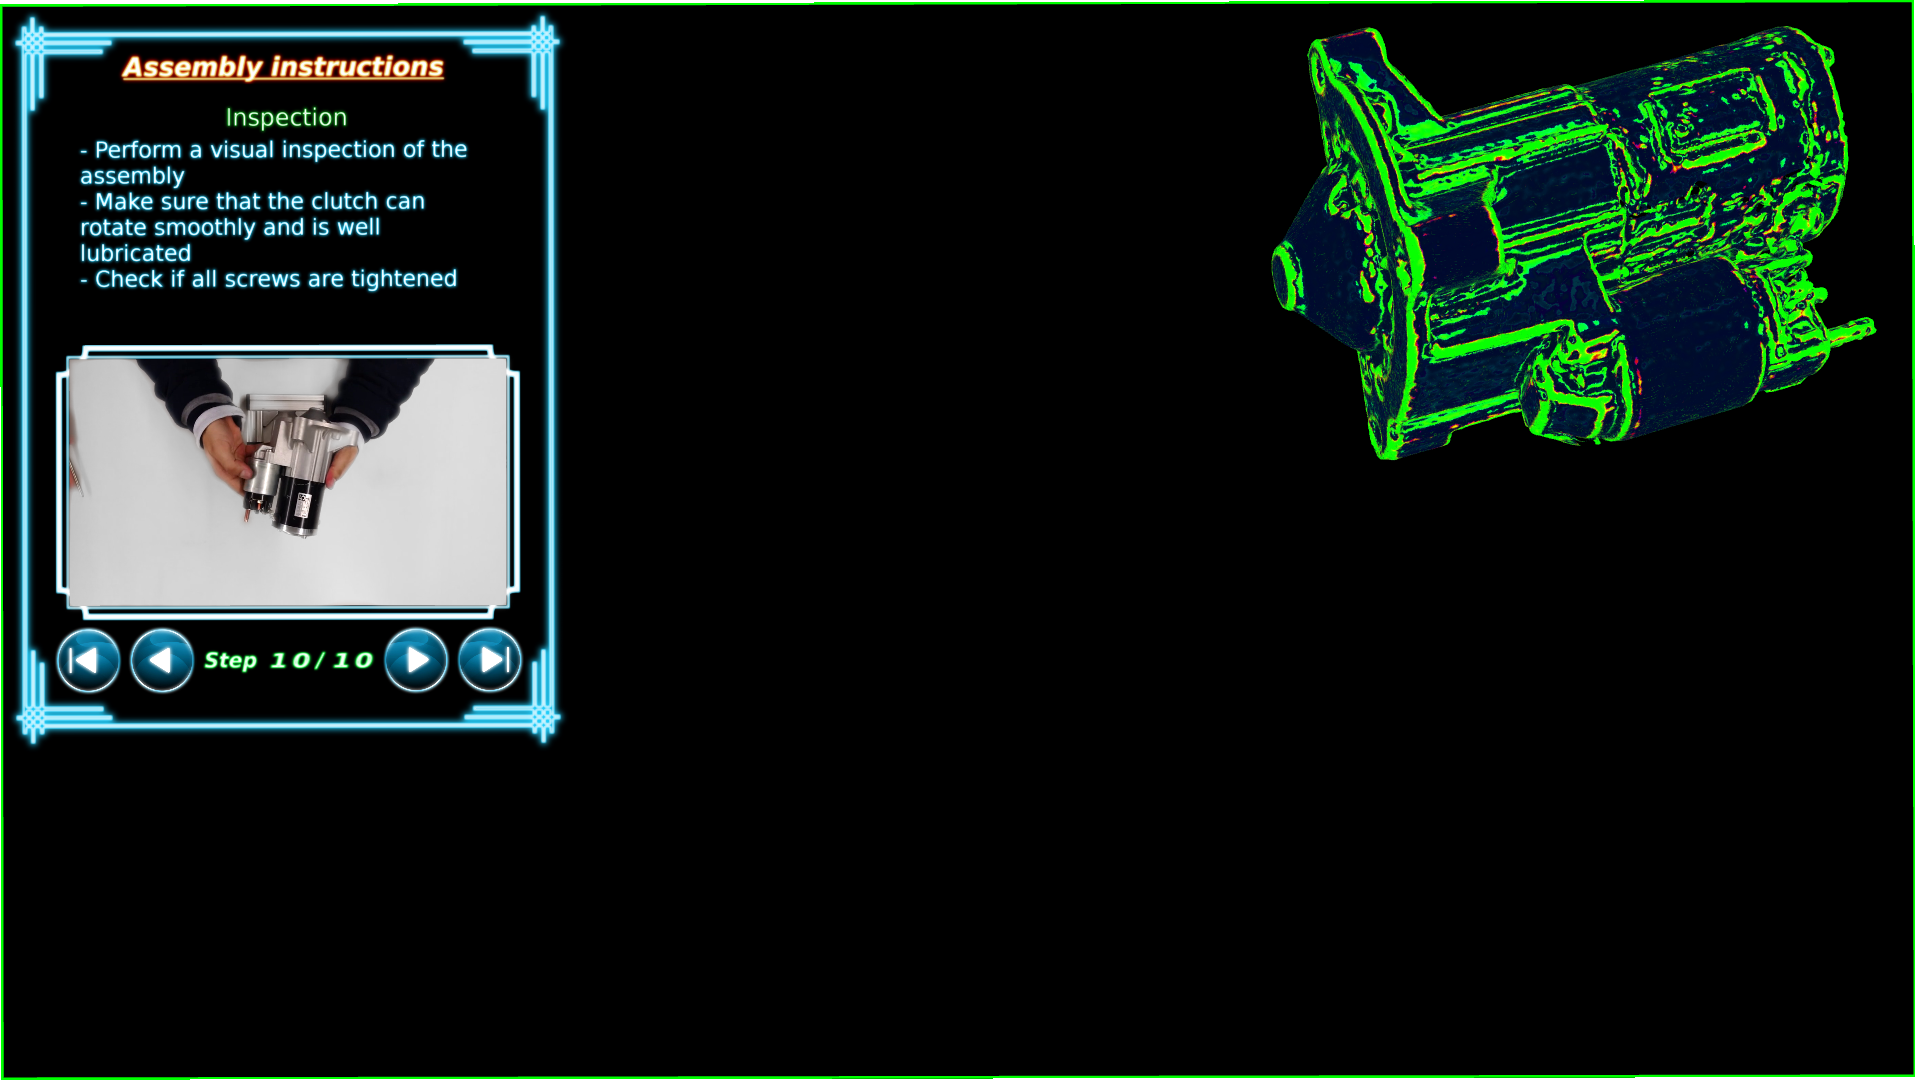
\includegraphics[width=0.99\linewidth]{scene-rendering}
	\caption{3D scene rendering using the Gazebo simulator}
	\label{fig:scene-rendering}
\end{figure}



\section{Human machine interface}\label{sec:human-machine-interaction}

The immersive \gls{hmi} system developed (shown in \cref{fig:scene-rendering,fig:human-machine-interface}) projects into the workspace detailed textual information of the current assembly task along with a video showing the operation being performed by an expert operator. Given the high variability of assembly / maintenance operations, the system was designed to decompose the assembly process into a set of small and concise operations. This allows to keep the operator focused on the current task and reduces the required projection area. Moreover, the operator can pause and move the video forwards and backwards, allowing him to inspect a given complex operation with more time.

The user interaction with the projected \gls{hmi} is done by analyzing the 3D point cloud sensor data that falls within a set of \glspl{roi}, that are shown in \cref{fig:interaction-rois} as 4 green cubes for navigating within the assembly steps (first, previous, next and last), 1 dark blue box for pausing / playing the video and 1 yellow box for the video seek functionality (examples of user interacting the the \gls{hmi} shown in \cref{fig:interaction-pause,fig:interaction-next,fig:interaction-seek}).

For ensuring robust detection of the user intentions, each \gls{roi} has a state machine that triggers its associated action only when a minimum number of points falls within the specified \gls{roi} boundaries (avoids sensor noise problems) and the user holds his finger within it for at least 0.25 seconds. Moreover, to avoid unintentionally triggering the same action several times, the user needs to remove and insert the finger into the \gls{roi} to request the action again.

When a \gls{roi} state machine activates its action, the 3D sensor data centroid (shown as spheres in \cref{fig:interaction-rois}) is computed for providing a visual debugging feedback of the \gls{hmi} state and also for being used in higher level perception, namely in the seek bar \gls{roi} (the vertical yellow box in \cref{fig:interaction-rois}), in which the seek time is computed considering the relative position of the finger within the \gls{roi} (the bottom of the \gls{roi} is associated with the start of the current video while the top corresponds to the end of the current video).

\begin{figure}[H]
	\begin{floatrow}[2]
		\ffigbox[\FBwidth]
		{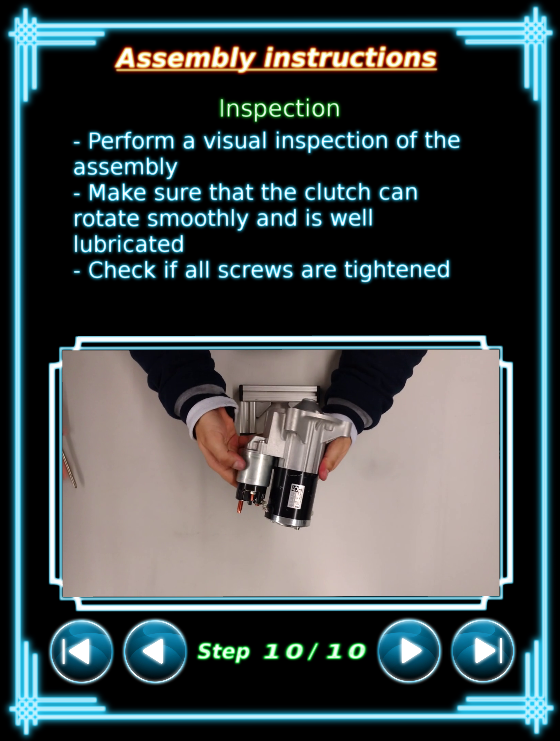
\includegraphics[height=.24\textheight]{human-machine-interface}}
		{\caption{Rendering of the human machine interface using Gazebo}\label{fig:human-machine-interface}}
		\ffigbox[\FBwidth]
		{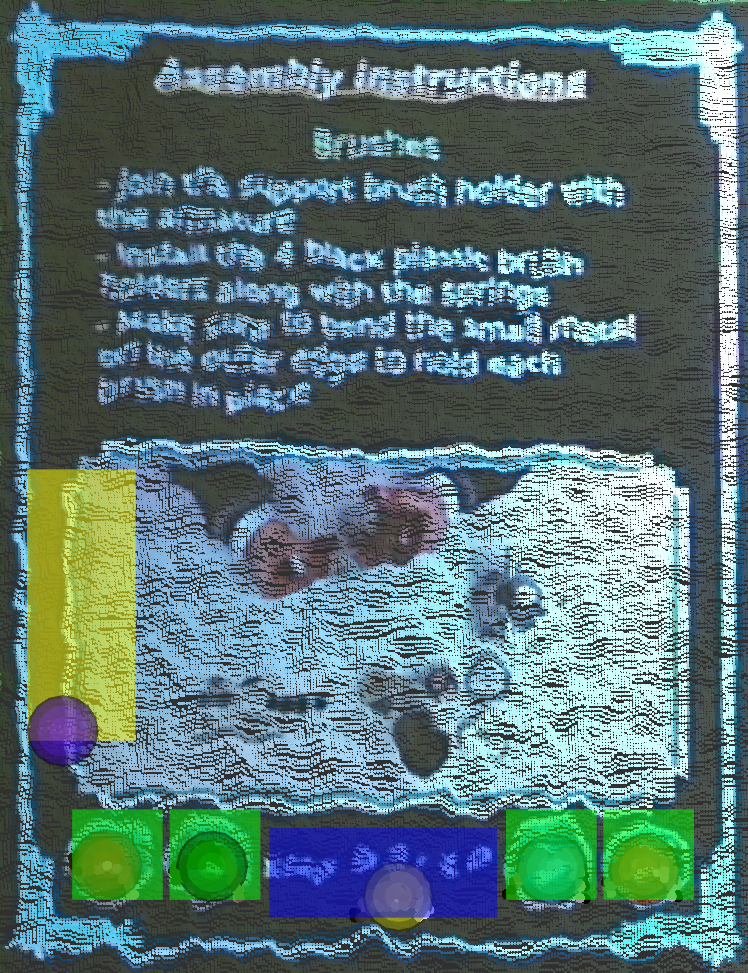
\includegraphics[height=.24\textheight]{interaction-rois}}
		{\caption{\glspl{roi} for the \gls{hmi} (overlaid on top of the Kinect 2 point cloud sensor data using Rviz)}\label{fig:interaction-rois}}
	\end{floatrow}
\end{figure}

\begin{figure}[ht]
	\begin{floatrow}[3]
		\ffigbox[\FBwidth]
		{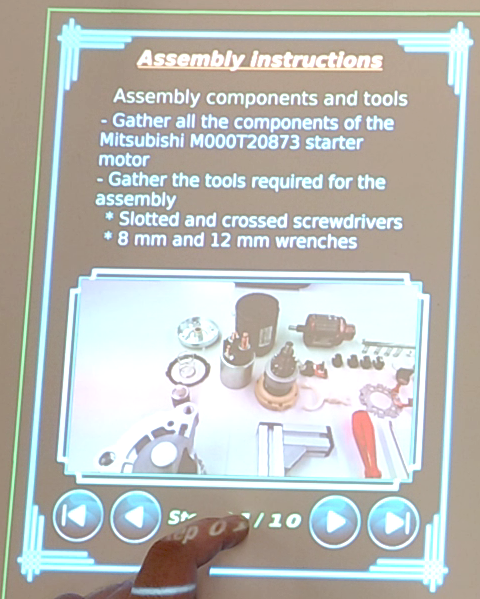
\includegraphics[height=.15\textheight]{interaction-pause}}
		{\caption{Example of video play / pause interaction}\label{fig:interaction-pause}}
		\ffigbox[\FBwidth]
		{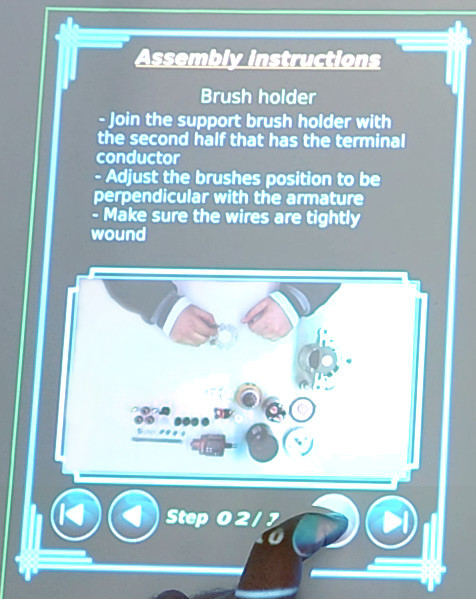
\includegraphics[height=.15\textheight]{interaction-next}}
		{\caption{Visual highlight of the request to move to the next assembly step}\label{fig:interaction-next}}
		\ffigbox[\FBwidth]
		{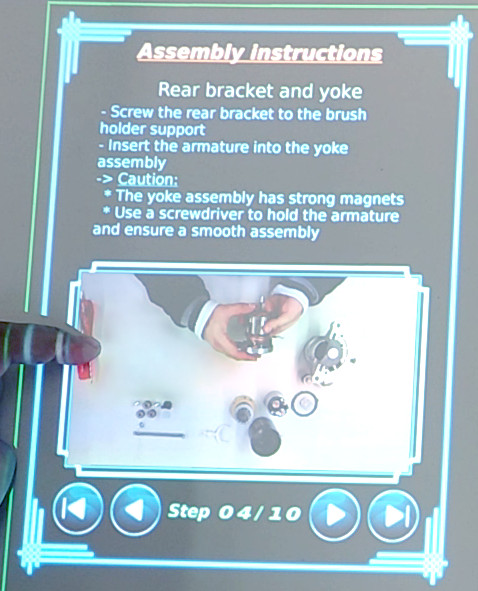
\includegraphics[height=.15\textheight]{interaction-seek-2}}
		{\caption{Example of video seek interaction}\label{fig:interaction-seek}}
	\end{floatrow}
\end{figure}


\section{Object 3D reconstruction}\label{sec:object-reconstruction}

For performing proper 3D rendering and also be able to estimate the 6 \gls{dof} pose of an object within the workspace, a 3D \gls{cad} or mesh model of the final product is required. Given the lack of public available \gls{cad} models for the Mitsubishi M000T20873 starter motor (shown in \cref{fig:starter-motor}), it was necessary to perform object 3D reconstruction. The 3D mesh model shown in \cref{fig:object-reconstruction} was generated using the David Laser 3D structured light system\footnote{\url{http://www.david-3d.com}}, and was built by surface matching algorithms using sensor data retrieved from 38 scans in which the starter motor was moved and rotated several times in order to capture enough sensor data to be able to reconstruct the entire surface. This particular object created some challenges for the structured light scanner because it contains polished metallic sections and also black coated surfaces. As such, it was necessary to capture the same object sections several times with different projector brightness and camera exposure times (the dark regions required the maximum projector brightness and very high exposure times while the polished sections required dimmer projector brightness and very short exposure times in order for the surface to be fully reconstructed). Moreover, for ensuring that the matching algorithms worked as expected, all captured point clouds needed to be manually cleaned using the David Laser scanning software before performing the alignment and reconstruction of the mesh model.

The last step of the assembly process includes a visual inspection stage performed by the operator in which it compares the final assembled product with a projected surface outline computed from the reconstructed mesh and overlaid on top of the physical object after its 6 \gls{dof} pose is estimated. The outline was computed using the curvature estimator available in MeshLab\footnote{\url{http://www.meshlab.net}}. Namely, the "Compute curvature principal directions" filter was used with the principal component analysis method and the mean curvature color mapping algorithm (result show in \cref{fig:object-reconstruction}). For improving the visibility of the outline, the color palette was remapped to show the high curvature regions (associated with surfaces boundaries) using the green color instead of red and the remaining intermediate curvatures were changed to very dark blue, for giving high contrast between the outline and the other surfaces. This was achieved by exporting the mesh to the .dae format (require by Gazebo for displaying colored models) with the color information separated to a .png texture. This way, it was possible to use Gimp\footnote{\url{https://www.gimp.org}} for remapping and enhance the mesh surface color outlines (as seen in \cref{fig:scene-rendering,fig:projection-mapping-3}).

\begin{figure}[!ht]
	\centering
	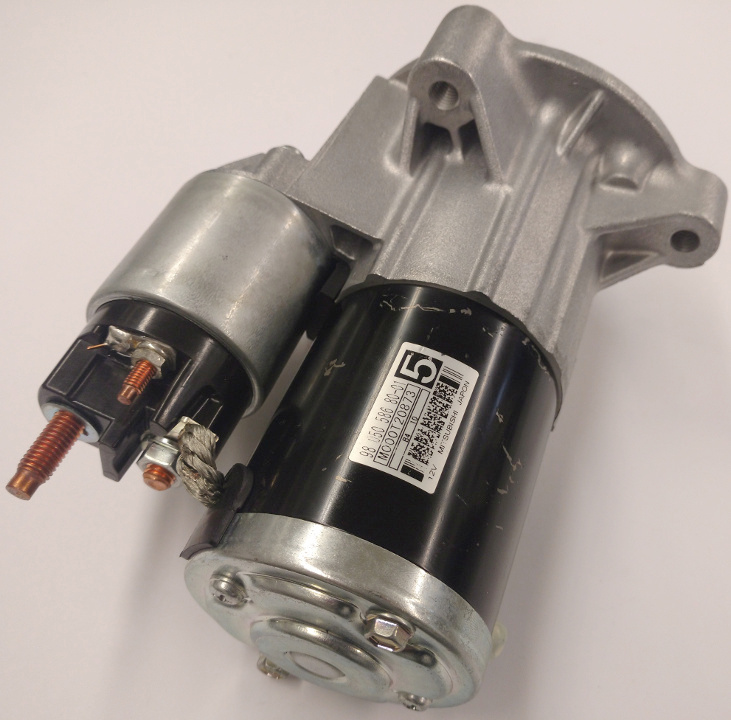
\includegraphics[height=.152\textheight]{mitsubishi-m000t20873-front}
	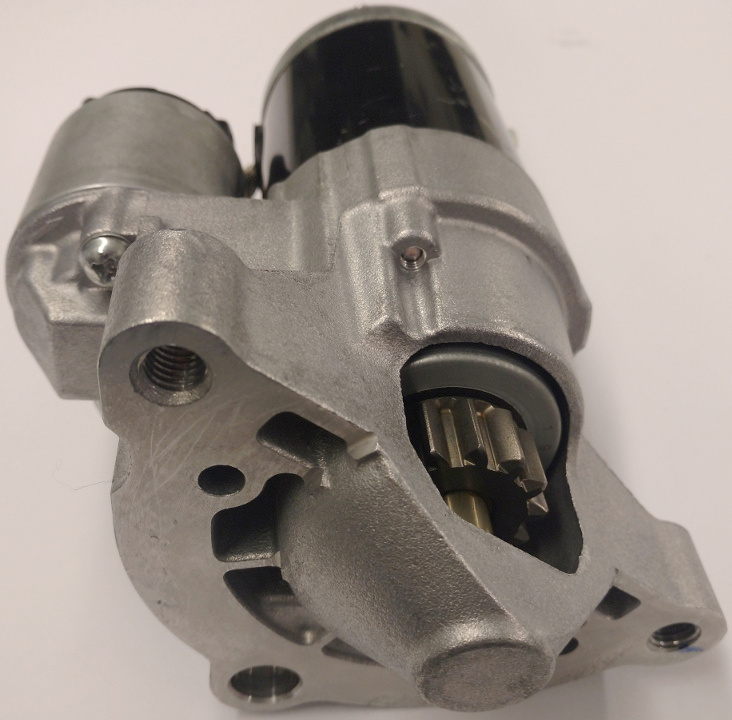
\includegraphics[height=.152\textheight]{mitsubishi-m000t20873-back}
	\caption{Mitsubishi M000T20873 starter motor}
	\label{fig:starter-motor}
\end{figure}

\begin{figure}[!ht]
	\centering
	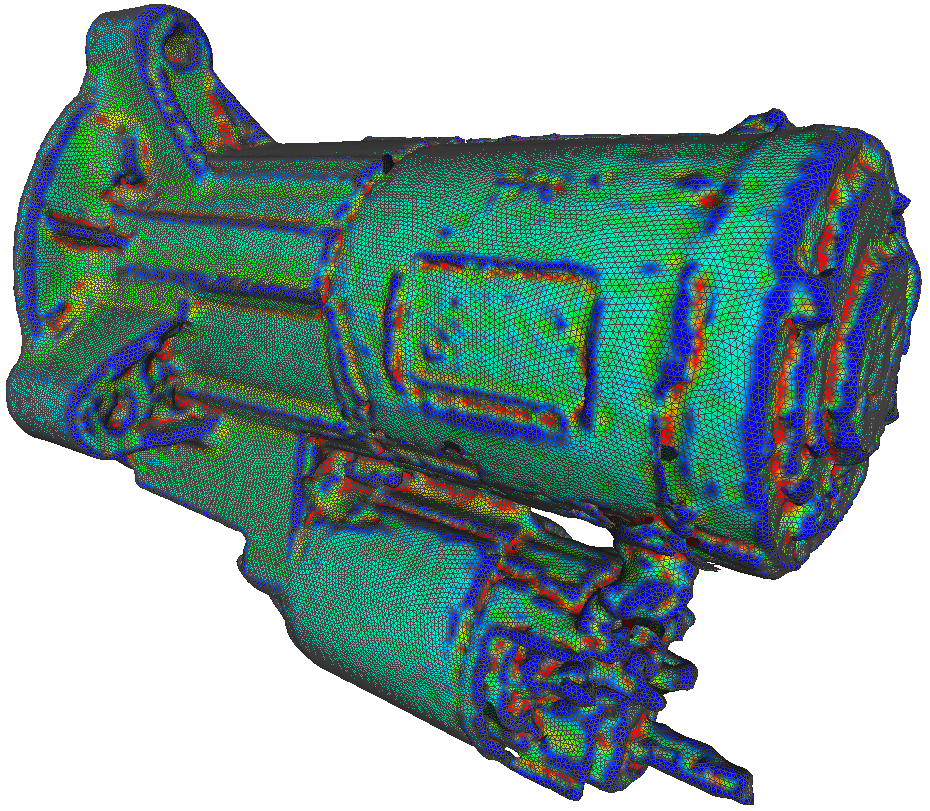
\includegraphics[height=.142\textheight]{object-reconstruction-front}
	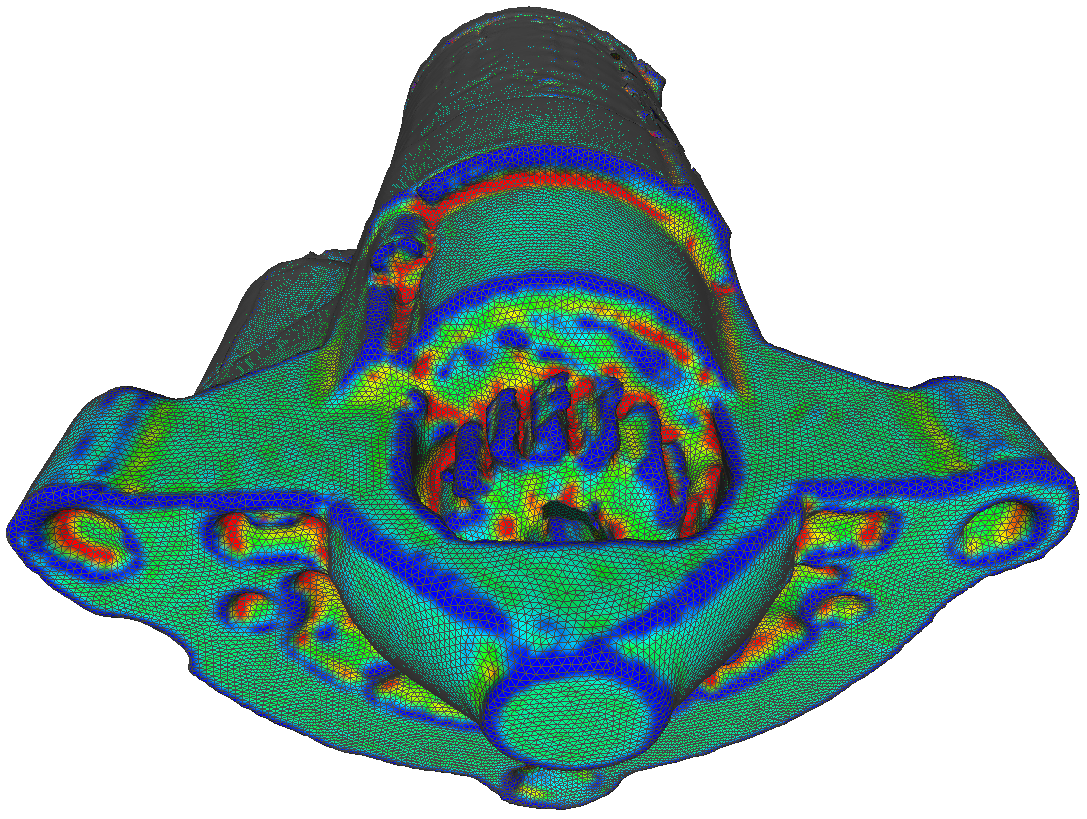
\includegraphics[height=.142\textheight]{object-reconstruction-back}
	\caption{3D model of the starter motor reconstructed using the David Laser structured light 3D scanner}
	\label{fig:object-reconstruction}
\end{figure}



\section{6 DoF pose estimation of objects}\label{sec:pose-estimation}

Robust and accurate estimation of the 6 \gls{dof} pose of objects is a requirement when virtual information must be overlaid on top of objects that may change their location over time. To achieve this goal, the 3D point cloud registration system (drl) described in \cite{Costa2016} was fine tuned for our table top use case.

We started by configuring the reference point cloud preprocessing pipeline to randomly select 3000 vertices of the starter engine reconstructed mesh (small green circles shown in \cref{fig:initial-pose-estimation}) and compute the \gls{sift} \cite{Lowe2004} keypoints (large yellow circles) and their associated \gls{fpfh} \cite{Rusu2009} feature descriptors.

Later on, we configured the runtime filtering stage of the drl system to segment the target object (starter motor) by extracting the points that were within a \gls{roi} specified in a calibrated frame on top of the table. The \gls{roi} defined the plausible space in which the object could be placed and also allowed to remove the points associated with the table. Moreover, for ensuring that the pose estimation would take less than 3 seconds, we also configured a random sample filter to downsample the point cloud within the \gls{roi} to 2500 points. Given that in this use case only a single object appears within the \gls{roi}, the clustering algorithms were not added to the drl runtime pipe. But they will be very useful in the future when we extend the proposed \gls{sar} system to provide contextual information and visual feedback for all the parts visible by the sensor (the clustering stage will then provide input for a object recognition module, which will determined which \gls{cad} is the best fit for each group of 3D points).

After finishing the setup of the preprocessing stage, we configured the initial alignment algorithms, namely, we fine tuned the \gls{sift} keypoint detector along with the \gls{fpfh} keypoint descriptor and the \gls{ransac} feature matcher. Later on, we fine tuned the \gls{icp} algorithm for refining the point cloud registration in order to achieve a 6 \gls{dof} pose estimation with hight accuracy (less than 2 mm or alignment error, as can be seen by the good overlap between the physical starter motor and its virtual outline displayed in \cref{fig:projection-mapping-3}).

The drl modules discussed earlier are enough for estimating the 6 \gls{dof} pose of objects, but for improving the efficiency of the drl we also configured the tracking and recovery matching pipelines. These two pipelines allow the definition of a set of cloud matchers that are fine tuned to align the sensor data by successively updating the 6 \gls{dof} pose of the object as new sensor data arrives. This allows to run the robust, but computationally expensive feature matching algorithms once, and then rely on dense point cloud matching algorithms to quickly and accurately update the object pose at the frame rate of the 3D sensor (up to 30 Hz, depending on the CPU used). The tracking pipeline was configured to rely on the \gls{icp} algorithm with the point-to-point metric with a search radius 0.07 m for establishing correspondences during the iterative matching process and with the maximum number of iterations set to 300. On the other hand, the recovery pipeline was fine tuned to use the \gls{icp} algorithm with the point-to-plane metric with the search radius and number of iterations increased to 0.2 m and 400 respectively. This approach of starting with robust feature matching algorithms and then rely on tracking algorithms with the sporadic usage of tracking recovery methods was critical for being able to track the object with a reasonable frame rate, which will be useful in the future when we extend the proposed \gls{sar} to monitor the operator actions for ensuring he is following the instructions and did not forget or misplaced assembly parts.

In \cref{fig:initial-pose-estimation} is shown an example of the estimation of the 6 \gls{dof} pose of the starter motor. The left image displays the overlay of the reference point cloud on top of the 3D sensor data in the previously estimated pose (before the operator occluded the part with its hand and move it to a new place) while the right image shows the updated pose after alignment, that correctly detected that the operator moved the part to the right and rotated it 90º clockwise.

\begin{figure}[!ht]
	\centering
	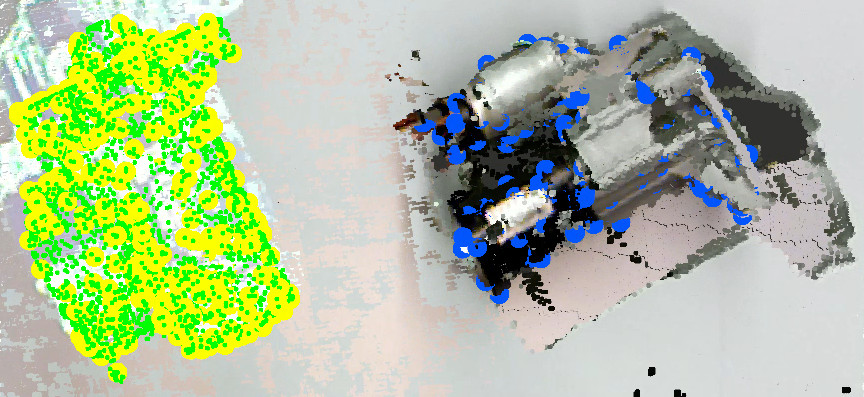
\includegraphics[height=.11\textheight]{initial-pose-estimation-2-before}
	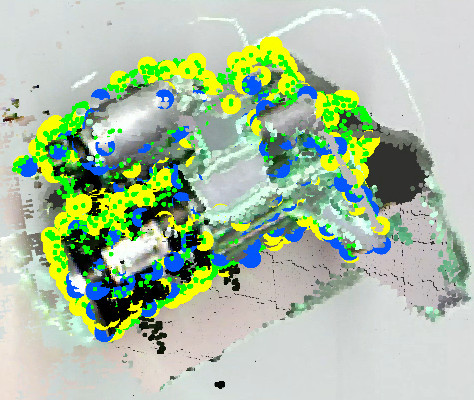
\includegraphics[height=.11\textheight]{initial-pose-estimation-2-after}
	\caption{Example of 6 DoF pose estimation of the assembled starter motor before (left) and after (right) the alignment of the 3D reconstructed mesh with the 3D sensor data}
	\label{fig:initial-pose-estimation}
\end{figure}
